\documentclass{standalone}
%
\usepackage{tikz}
\usetikzlibrary{backgrounds,
	arrows.meta,
	calc,
	decorations.pathmorphing,
shapes.callouts}
\usepackage{tkz-euclide}
%
%\usetkzobj{all}
\usepackage{xcolor}
\usepackage{ifthen}
%
\definecolor{space}{HTML}{1F2C4E}
\definecolor{earth}{HTML}{0089FA}
\definecolor{dida}{HTML}{FFDE00}
\definecolor{title}{HTML}{FBA706}
\definecolor{spacetime}{HTML}{0CF508}
%
\usepackage{fontspec}
\setmainfont{Open Dyslexic}
%
\title{Lo spaziotempo}
\begin{document}
	\tikzset{
		partial ellipse/.style args = {#1:#2:#3}{insert path={+ (#1:#3) arc (#1:#2:#3)}},
		notice/.style  = { draw, ellipse callout, callout relative pointer={#1} },
	}
	\begin{tikzpicture}[background rectangle/.style={fill=white},show background rectangle,>={[inset=0,angle'=27]Stealth}]
		%title
		\draw [black,ultra thick,fill=title] (0,9.8) rectangle (30,16.8);
		\node at (15,14.8) {\textcolor{black}{\fontsize{90}{91}\selectfont Analogie}};
		\node at (15,11.8) {\textcolor{black}{\fontsize{90}{91}\selectfont spaziotemporali}};
		%
		\begin{scope}[shift={(0,5)}]
			\draw [ultra thick, fill=earth] (20.5,4) rectangle (25.5,-4);
			\node at (23,0) {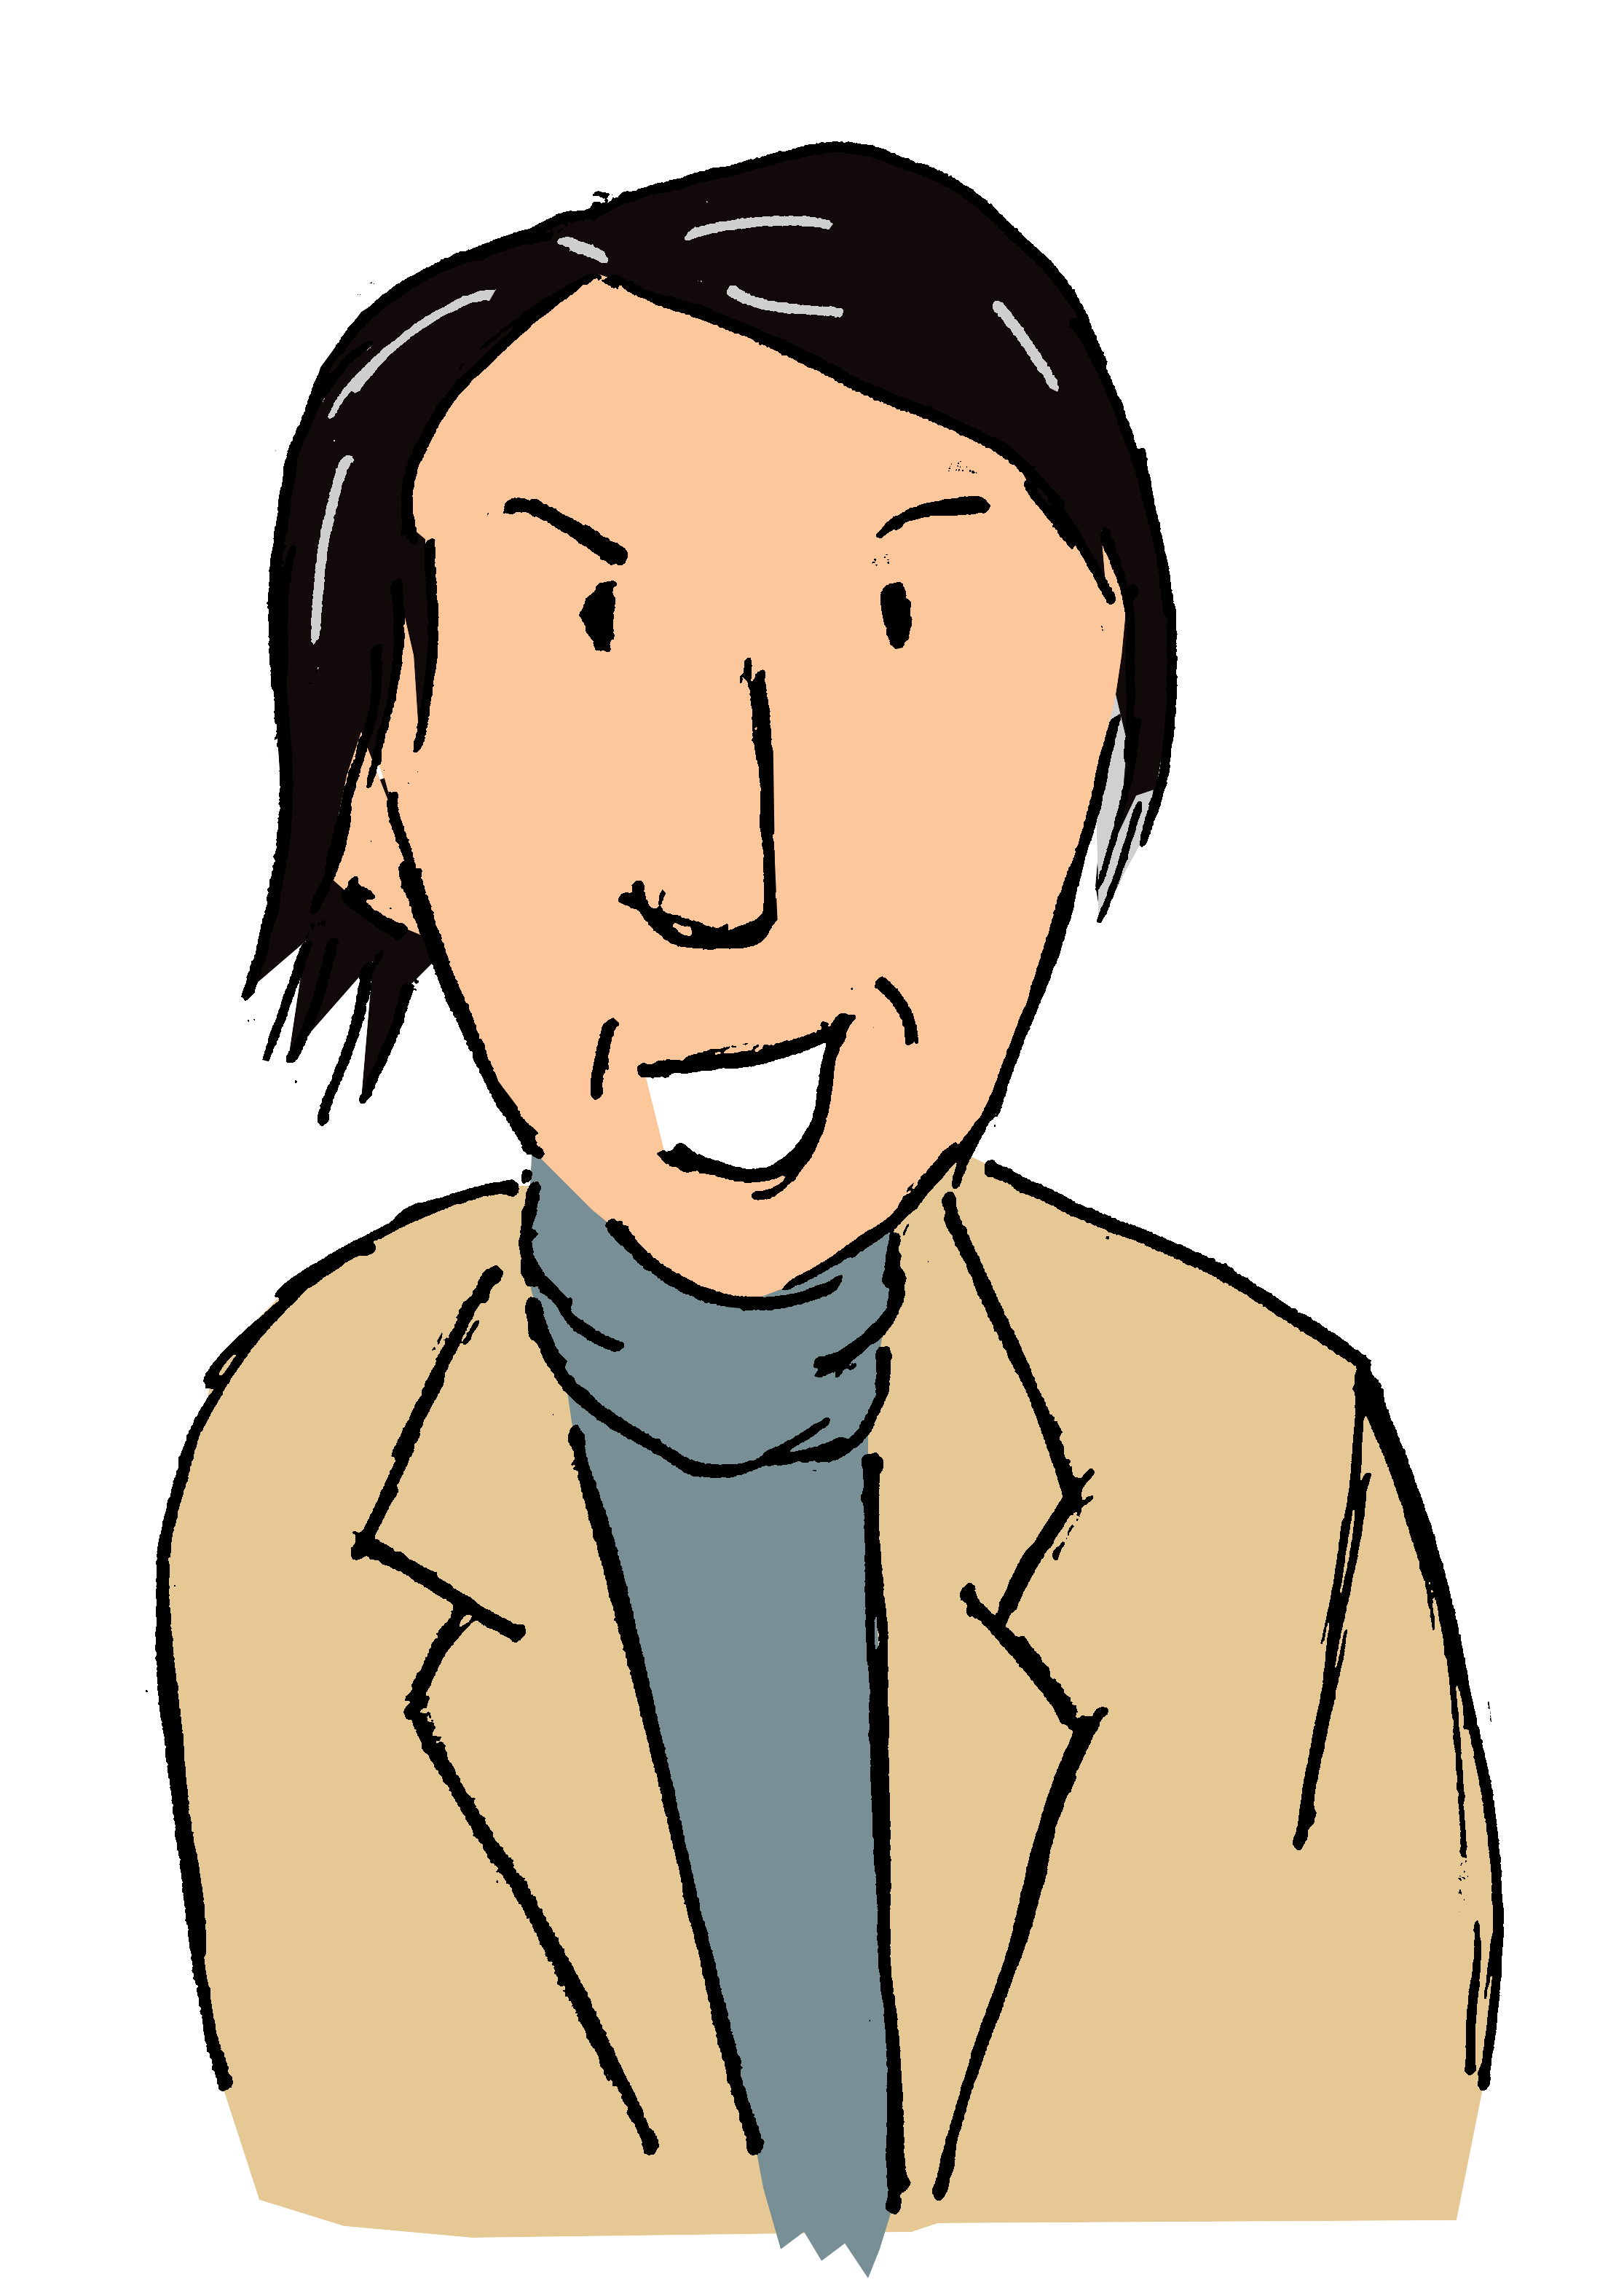
\includegraphics[width=5cm]{carl_sagan}};
			\node (example-textwidth-2) [notice={(3,0.5)}, ultra thick, right, align=center, text width=12cm, color=black, fill=white, font=\fontsize{23pt}{24pt}\selectfont] at (1,-1) {Benvenuti! Oggi parliamo di un concetto molto importante per la relatività speciale e generale: lo spaziotempo.};
		\end{scope}
		%
		\begin{scope}[shift={(0,-4)}]
			\draw [ultra thick, fill=earth] (4.5,4) rectangle (9.5,-4);
			\node at (7,0) {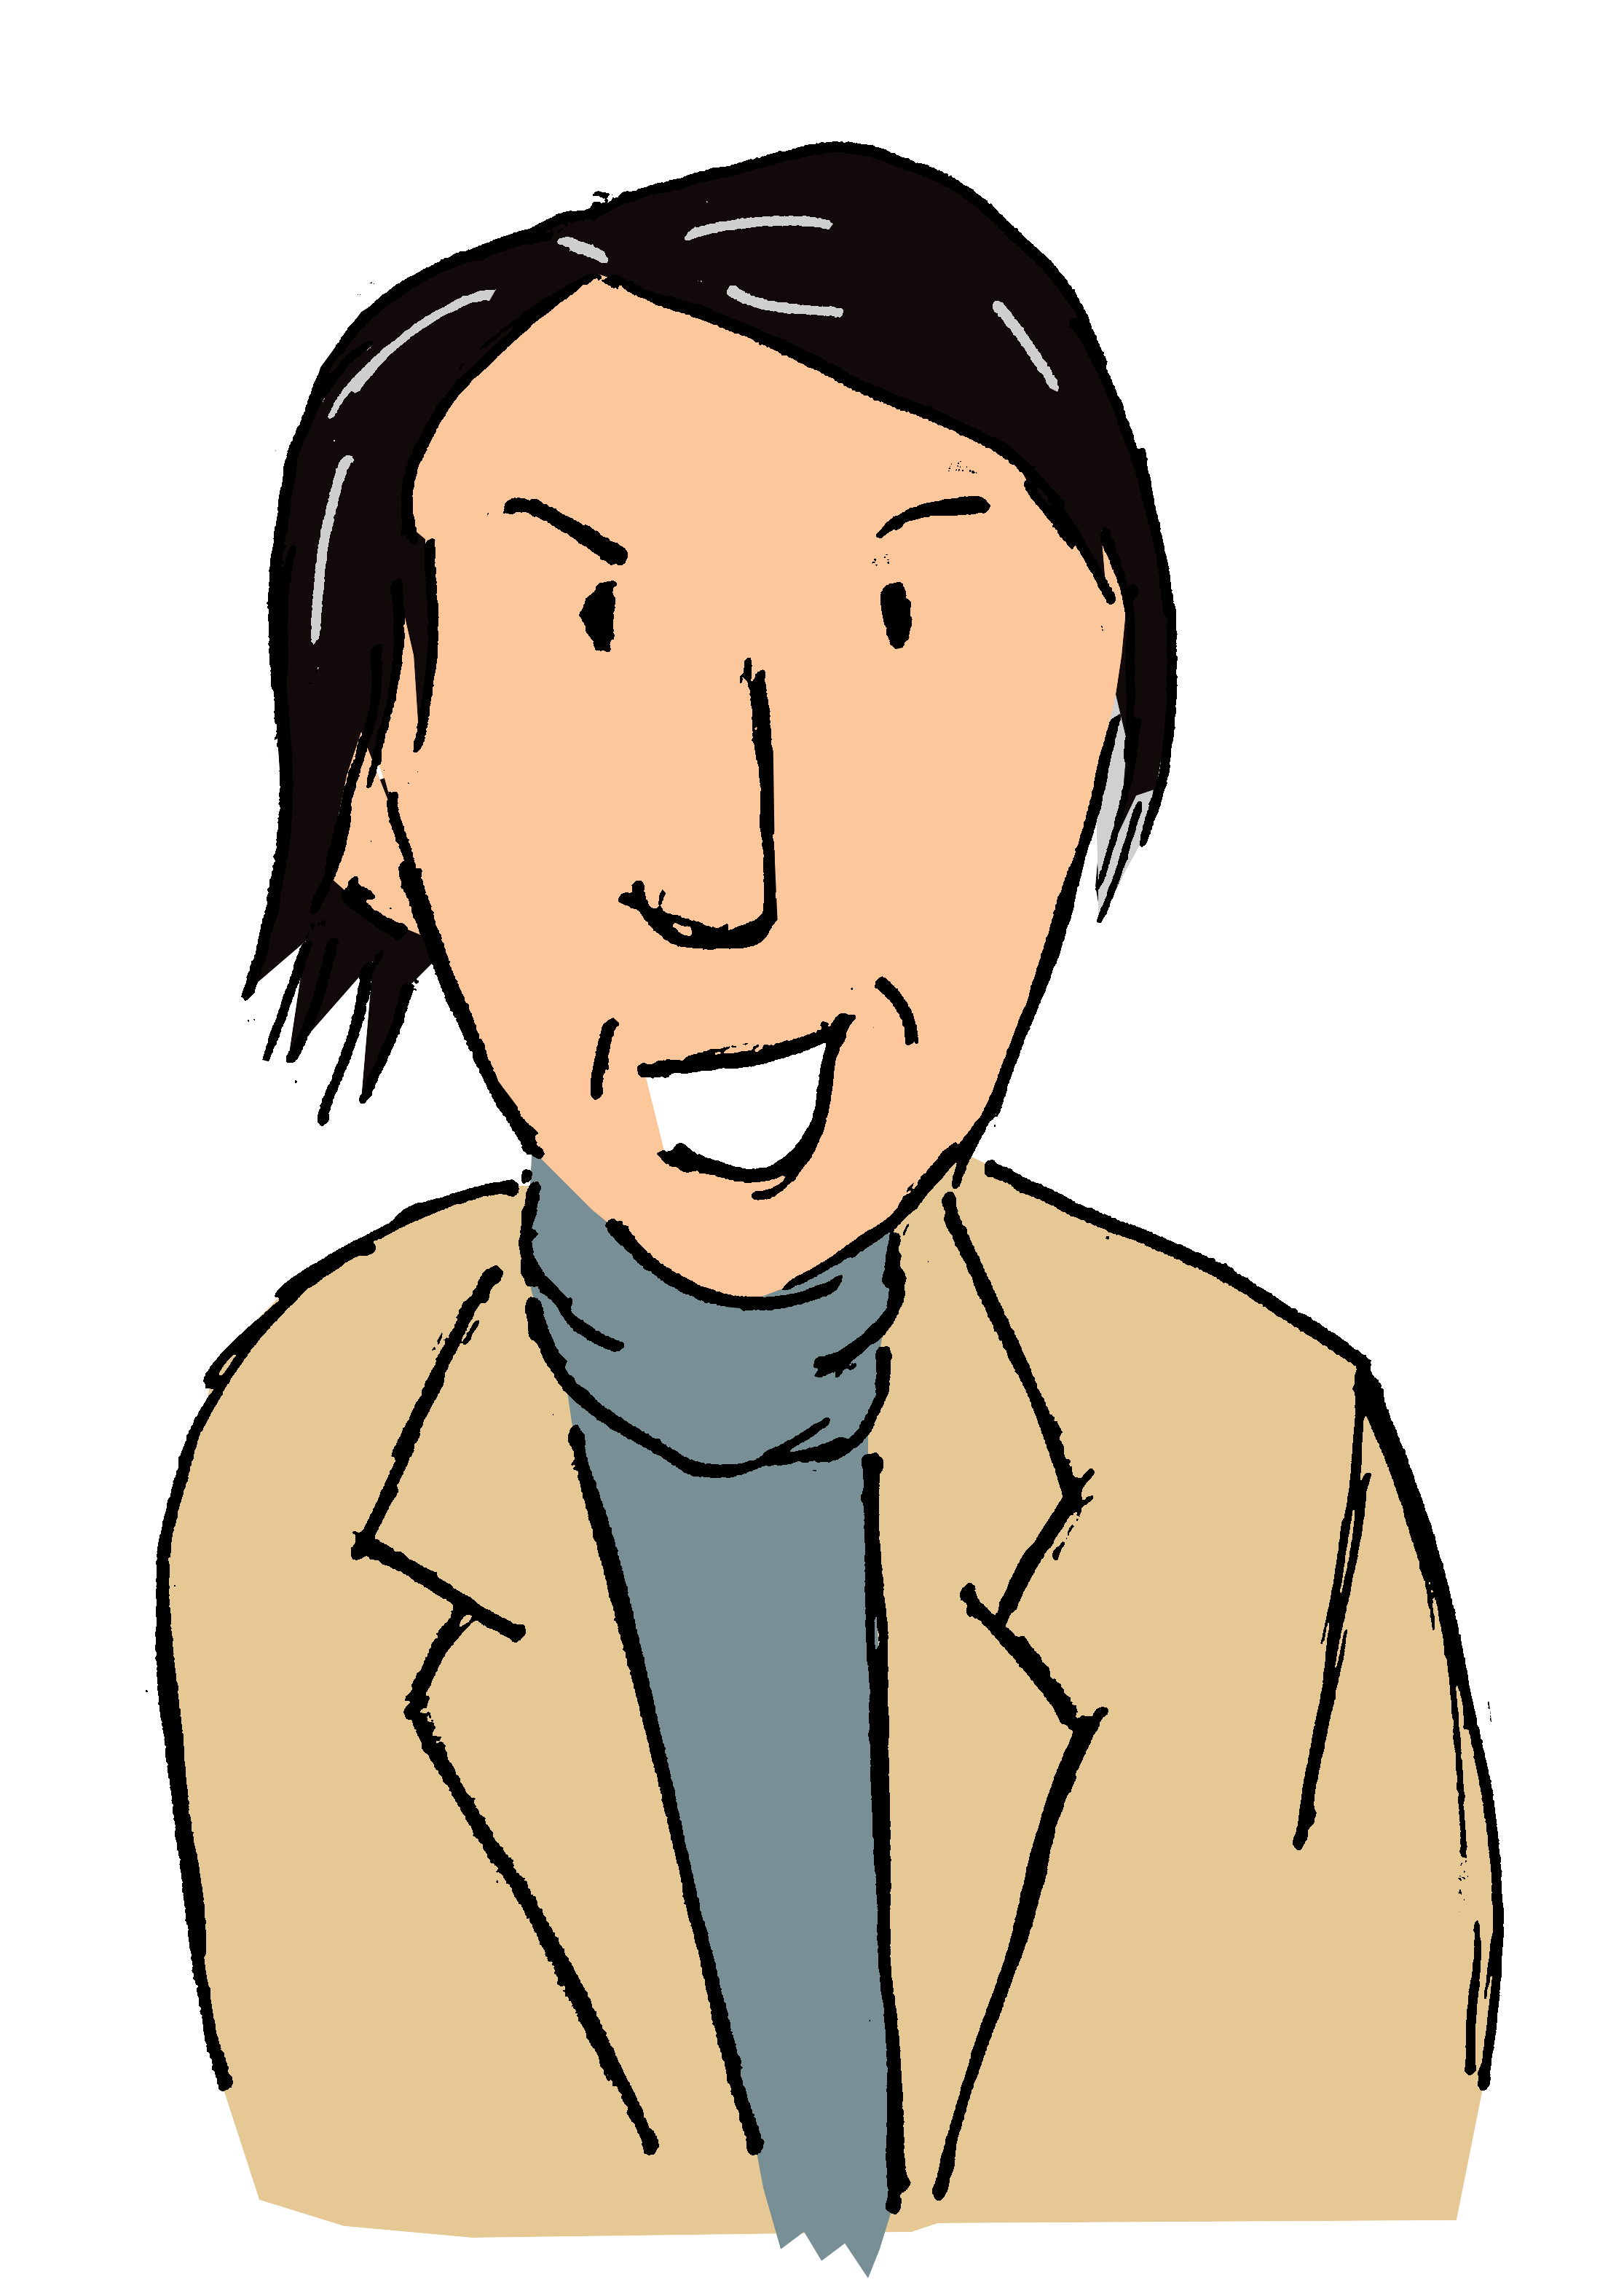
\includegraphics[width=5cm]{carl_sagan}};
			\node (example-textwidth-2) [notice={(-3,0.5)}, ultra thick, right, align=center, text width=12cm, color=black, fill=white, font=\fontsize{23pt}{24pt}\selectfont] at (12,-1) {Uno dei modelli per raccontare la teoria della relatività generale più utilizzati è quello del telo elastico con al centro una pallina che lo deforma.};
			%flamm paraboloid
			\begin{scope}[shift={(14,-14)}]
				%
				\draw (-0.1,-2.9) to[out=90,in=275] (-0.9,8.3);
				\draw (-0.6,-2.7) to[out=98,in=300] (-5.1,7.8);
				\draw (-1.1,-2.7) to[out=100,in=314] (-8.7,6.7);
				\draw (-1.3,-2.4) to[out=120,in=325] (-5.9,1.9) to[out=148,in=335] (-11.2,4.9);
				\draw (-1.6,-2.4) to[out=130,in=330] (-4.9,0.1) to[out=150,in=340] (-12,2.9);
				%
				\draw (0.3,-2.9) to[out=81,in=250] (3.5,8.1);
				\draw (0.8,-2.6) to[out=76,in=231] (7.4,7.2);
				\draw (1.4,-2.5) to[out=65,in=214] (10.5,5.6);
				\draw (1.7,-2.4) to[out=75,in=210] (4.85,0.5) to[out=20,in=180] (11.9,2.4);
				%
				\draw (0,-1.8) [partial ellipse=0:180:2.1 and 1];
				\draw (0,-1.2) [partial ellipse=0:180:2.8 and 1.3];
				\draw (0,-0.6) [partial ellipse=0:180:3.5 and 1.6];
				\draw (0,0) [partial ellipse=0:180:4.2 and 1.8];
				\draw (0,0.3) [partial ellipse=0:180:4.9 and 2.1];
				%
				\draw[fill=red] (0,0) circle (2.9cm);
				%
				\draw (-1.6,-2.4) to[out=150,in=330] (-3.5,-1) to[out=160,in=350] (-10.8,0.7);
				\draw (-1.3,-2.6) to[out=165,in=330] (-2.9,-1.4) to[out=165,in=360] (-7.8,-1);
				\draw (-1,-2.7) to[out=130,in=330] (-2,-1.6) to[out=160,in=30] (-4.6,-1.9);
				\draw (-0.5,-2.85) to[out=90,in=350] (-1,-1.8) to[out=160,in=40] (-1.8,-2.25);
				%
				\draw (1.5,-2.5) to[out=80,in=214] (3.5,-1) to[out=20,in=180] (9,-0.5);
				\draw (0.65,-2.8) to[out=80,in=214] (1.7,-1.7) to[out=20,in=170] (5.2,-1.8);
				\draw (0.1,-2.9) to [out=88,in=250] (0.3,-1.8) to[out=20,in=140] (1,-2.3);
				%
				\draw (0,-1.8) [partial ellipse=180:360:2.1 and 1];
				\draw (0,-1.2) [partial ellipse=180:360:2.8 and 1.3];
				\draw (0,-0.6) [partial ellipse=180:360:3.5 and 1.6];
				\draw (0,0) [partial ellipse=180:360:4.2 and 1.8];
				\draw (0,0.3) [partial ellipse=180:360:4.9 and 2.1];
				\draw (0,0.6) ellipse (5.6cm and 2.4cm);
				\draw (0,0.9) ellipse (6.3cm and 2.7cm);
				\draw (0,1.2) ellipse (7cm and 3cm);
				\draw (0,1.5) ellipse (7.7cm and 3.3cm);
				\draw (0,1.8) ellipse (8.5cm and 3.7cm);
				\draw (0,2.1) ellipse (9.3cm and 4.1cm);
				\draw (0,2.4) ellipse (10.2cm and 4.5cm);
				\draw (0,2.7) ellipse (11.1cm and 4.9cm);
				\draw (0,3) ellipse (12cm and 5.3cm);
			\end{scope}
		\end{scope}
		%dida
		\begin{scope}[shift={(0,-24)}]
			%
			\draw [fill=dida, ultra thick] (1,2.5) rectangle (27.5,-2.5);
			\node (example-textwidth-2) [right, align=left, text width=26cm, color=black, font=\fontsize{23pt}{24pt}\selectfont] at (1.5,0) {Questo permette di mostrare come palline più piccole "orbitino" intorno alla palla più grande al centro in un modo simile ai pianeti, almeno fino a che l'attrito non ha ragione del moto circolare, rallentando le palline che quindi cadono dentro la "sacca gravitazionale".};
		\end{scope}
		%
		%flamm paraboloid
		\begin{scope}[shift={(14,-37)}]
			%
			\draw (-0.1,-2.9) to[out=90,in=275] (-0.9,8.3);
			\draw (-0.6,-2.7) to[out=98,in=300] (-5.1,7.8);
			\draw (-1.1,-2.7) to[out=100,in=314] (-8.7,6.7);
			\draw (-1.3,-2.4) to[out=120,in=325] (-5.9,1.9) to[out=148,in=335] (-11.2,4.9);
			\draw (-1.6,-2.4) to[out=130,in=330] (-4.9,0.1) to[out=150,in=340] (-12,2.9);
			%
			\draw (0.3,-2.9) to[out=81,in=250] (3.5,8.1);
			\draw (0.8,-2.6) to[out=76,in=231] (7.4,7.2);
			\draw (1.4,-2.5) to[out=65,in=214] (10.5,5.6);
			\draw (1.7,-2.4) to[out=75,in=210] (4.85,0.5) to[out=20,in=180] (11.9,2.4);
			%
			\draw (0,-1.8) [partial ellipse=0:180:2.1 and 1];
			\draw (0,-1.2) [partial ellipse=0:180:2.8 and 1.3];
			\draw (0,-0.6) [partial ellipse=0:180:3.5 and 1.6];
			\draw (0,0) [partial ellipse=0:180:4.2 and 1.8];
			\draw (0,0.3) [partial ellipse=0:180:4.9 and 2.1];
			%
			\draw[fill=red] (0,0) circle (2.9cm);
			%
			\draw (-1.6,-2.4) to[out=150,in=330] (-3.5,-1) to[out=160,in=350] (-10.8,0.7);
			\draw (-1.3,-2.6) to[out=165,in=330] (-2.9,-1.4) to[out=165,in=360] (-7.8,-1);
			\draw (-1,-2.7) to[out=130,in=330] (-2,-1.6) to[out=160,in=30] (-4.6,-1.9);
			\draw (-0.5,-2.85) to[out=90,in=350] (-1,-1.8) to[out=160,in=40] (-1.8,-2.25);
			%
			\draw (1.5,-2.5) to[out=80,in=214] (3.5,-1) to[out=20,in=180] (9,-0.5);
			\draw (0.65,-2.8) to[out=80,in=214] (1.7,-1.7) to[out=20,in=170] (5.2,-1.8);
			\draw (0.1,-2.9) to [out=88,in=250] (0.3,-1.8) to[out=20,in=140] (1,-2.3);
			%
			\draw (0,-1.8) [partial ellipse=180:360:2.1 and 1];
			\draw (0,-1.2) [partial ellipse=180:360:2.8 and 1.3];
			\draw (0,-0.6) [partial ellipse=180:360:3.5 and 1.6];
			\draw (0,0) [partial ellipse=180:360:4.2 and 1.8];
			\draw (0,0.3) [partial ellipse=180:360:4.9 and 2.1];
			\draw (0,0.6) ellipse (5.6cm and 2.4cm);
			\draw (0,0.9) ellipse (6.3cm and 2.7cm);
			\draw (0,1.2) ellipse (7cm and 3cm);
			\draw (0,1.5) ellipse (7.7cm and 3.3cm);
			\draw (0,1.8) ellipse (8.5cm and 3.7cm);
			\draw (0,2.1) ellipse (9.3cm and 4.1cm);
			\draw (0,2.4) ellipse (10.2cm and 4.5cm);
			\draw (0,2.7) ellipse (11.1cm and 4.9cm);
			\draw (0,3) ellipse (12cm and 5.3cm);
		\end{scope}
		%
		\begin{scope}[shift={(0,-45)}]
			\draw [ultra thick, fill=earth] (20.5,4) rectangle (25.5,-4);
			\node at (23,0) {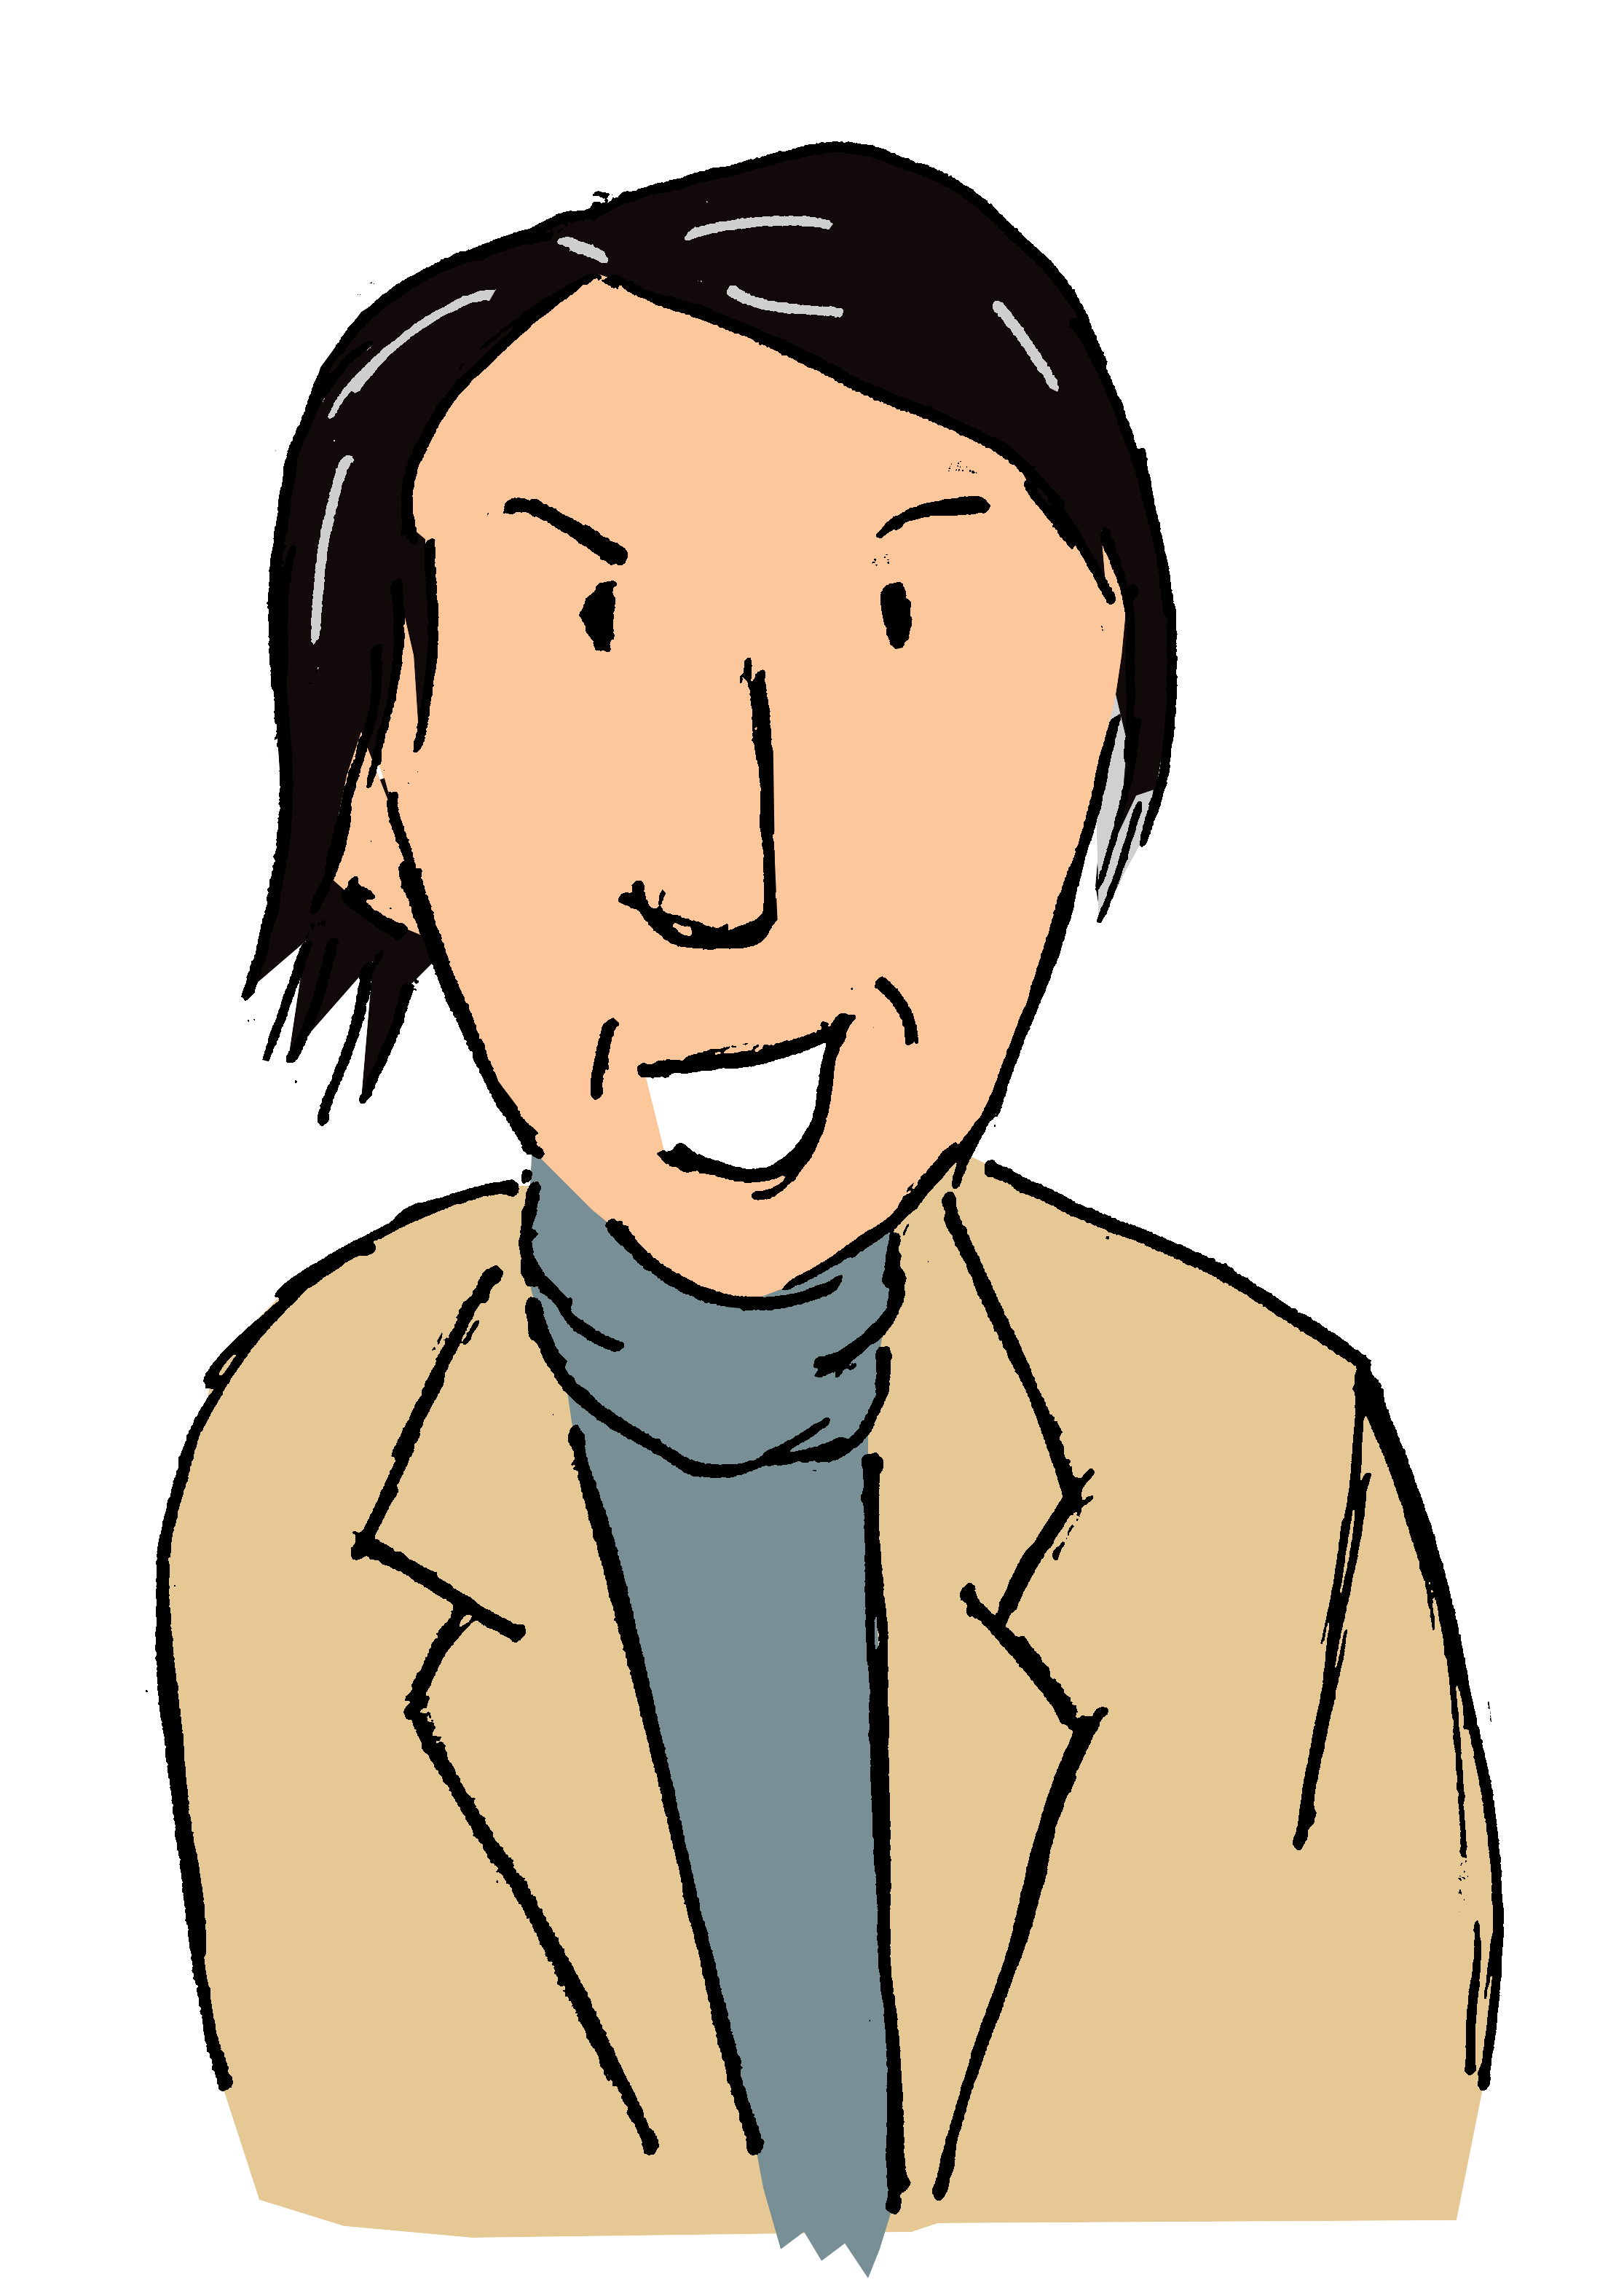
\includegraphics[width=5cm]{carl_sagan}};
			\node (example-textwidth-2) [notice={(3,0.5)}, ultra thick, right, align=center, text width=12cm, color=black, fill=white, font=\fontsize{23pt}{24pt}\selectfont] at (1,-1) {Questo modo "concreto" di vedere la relatività generale è diretta conseguenza del modo matematico "visuale" generato dai diagrammi di incorporamento e dai parabolodi di Flamm.};
		\end{scope}
		%
		\begin{scope}[shift={(0,-56)}]
			\draw [ultra thick, fill=earth] (4.5,4) rectangle (9.5,-4);
			\node at (7,0) {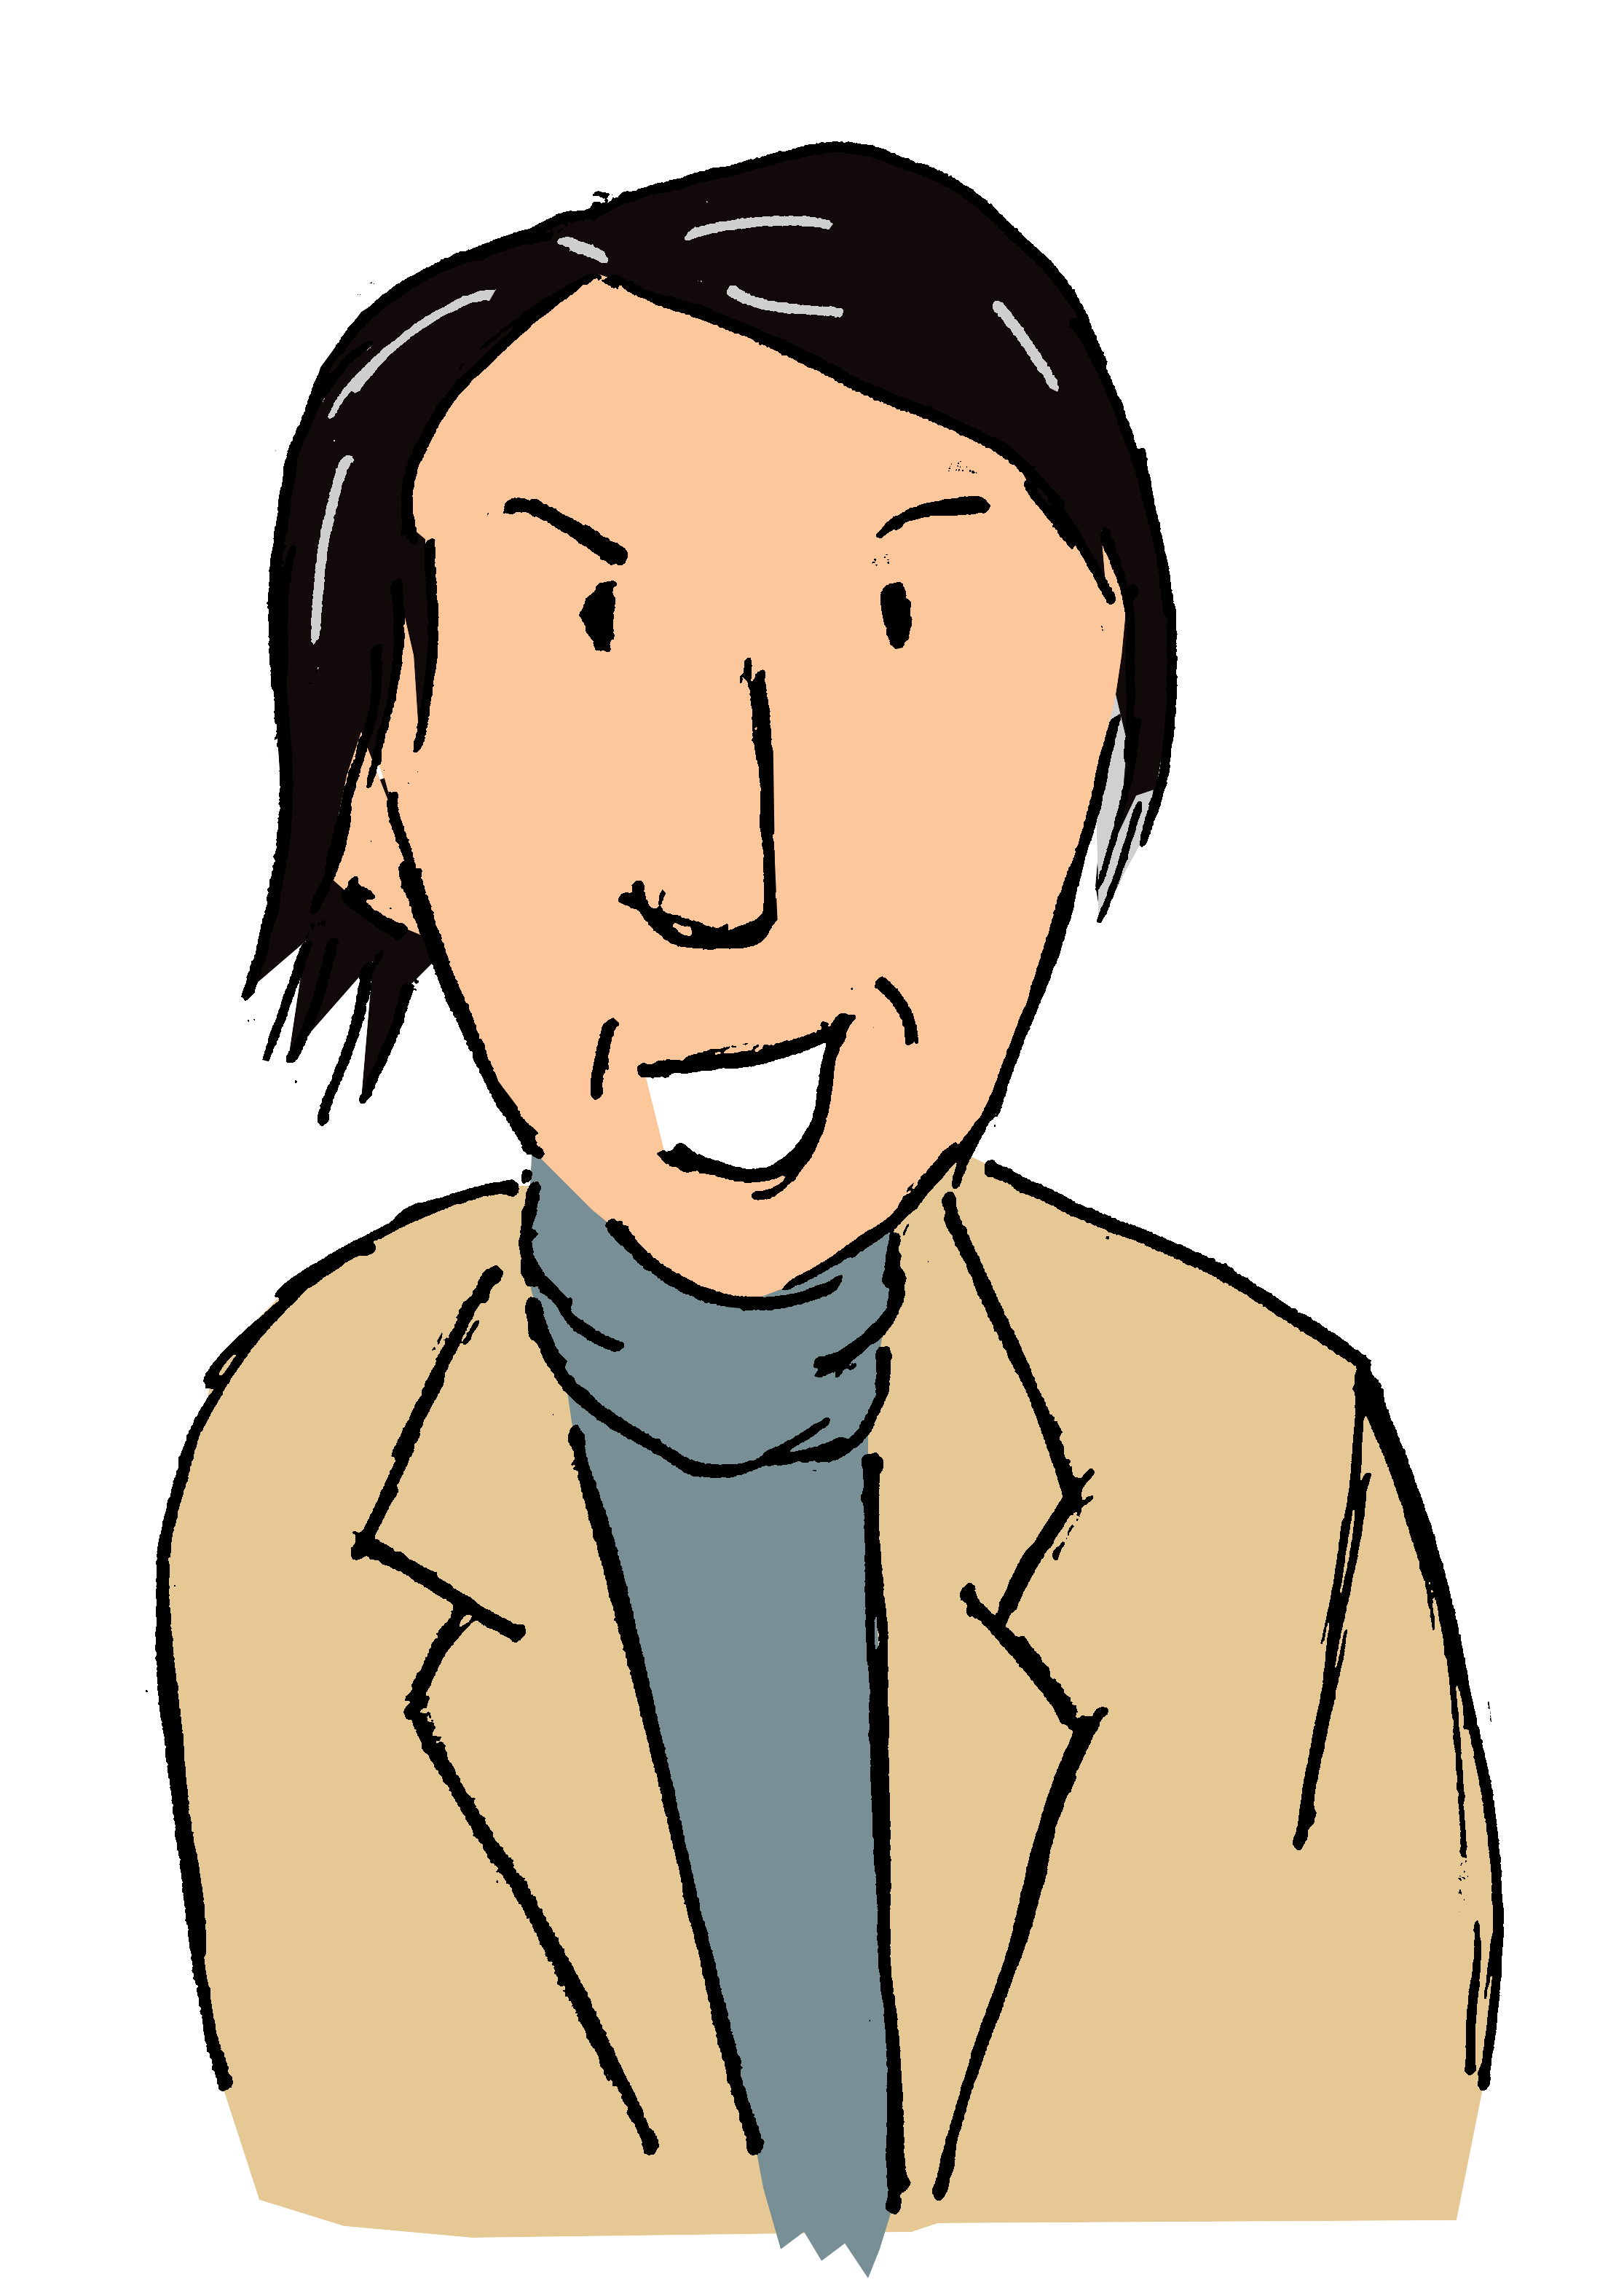
\includegraphics[width=5cm]{carl_sagan}};
			\node (example-textwidth-2) [notice={(-3,0.5)}, ultra thick, right, align=center, text width=12cm, color=black, fill=white, font=\fontsize{23pt}{24pt}\selectfont] at (12,-1) {Esiste, però, un metodo alternativo per raccontare la deformazione dello spaziotempo. Vediamolo insieme.};
		\end{scope}
		%
		\begin{scope}[shift={(0,-61)}]
			\draw[fill=space,ultra thick] (0.5,0) rectangle (28,-12);
			%
			\node (example-textwidth-2) [right, align=left, text width=26cm, color=white, font=\fontsize{23pt}{24pt}\selectfont] at (1.5,-3) {Supponiamo di voler andare da Ottawa a Venezia in aereo. Questo, che si sposta relativamente vicino alla superficie del pianeta, compirà un arco di circonferenza per andare dalla cittadina canadese fino a quella italiana, invece di prendere la retta che collega direttamente le due città.};
			\draw [color=white, ultra thick] (3,-10) -- (15,-10);
			\draw (9,-10) [color=white,ultra thick,partial ellipse=180:0:6 and 3];
			\node at (3,-11) {\textcolor{white}{\fontsize{23}{24}\selectfont Ottawa}};
			\node at (15,-11) {\textcolor{white}{\fontsize{23}{24}\selectfont Venezia}};
		\end{scope}
		%
		%
		\begin{scope}[shift={(0,-78)}]
			\draw [ultra thick, fill=earth] (20.5,4) rectangle (25.5,-4);
			\node at (23,0) {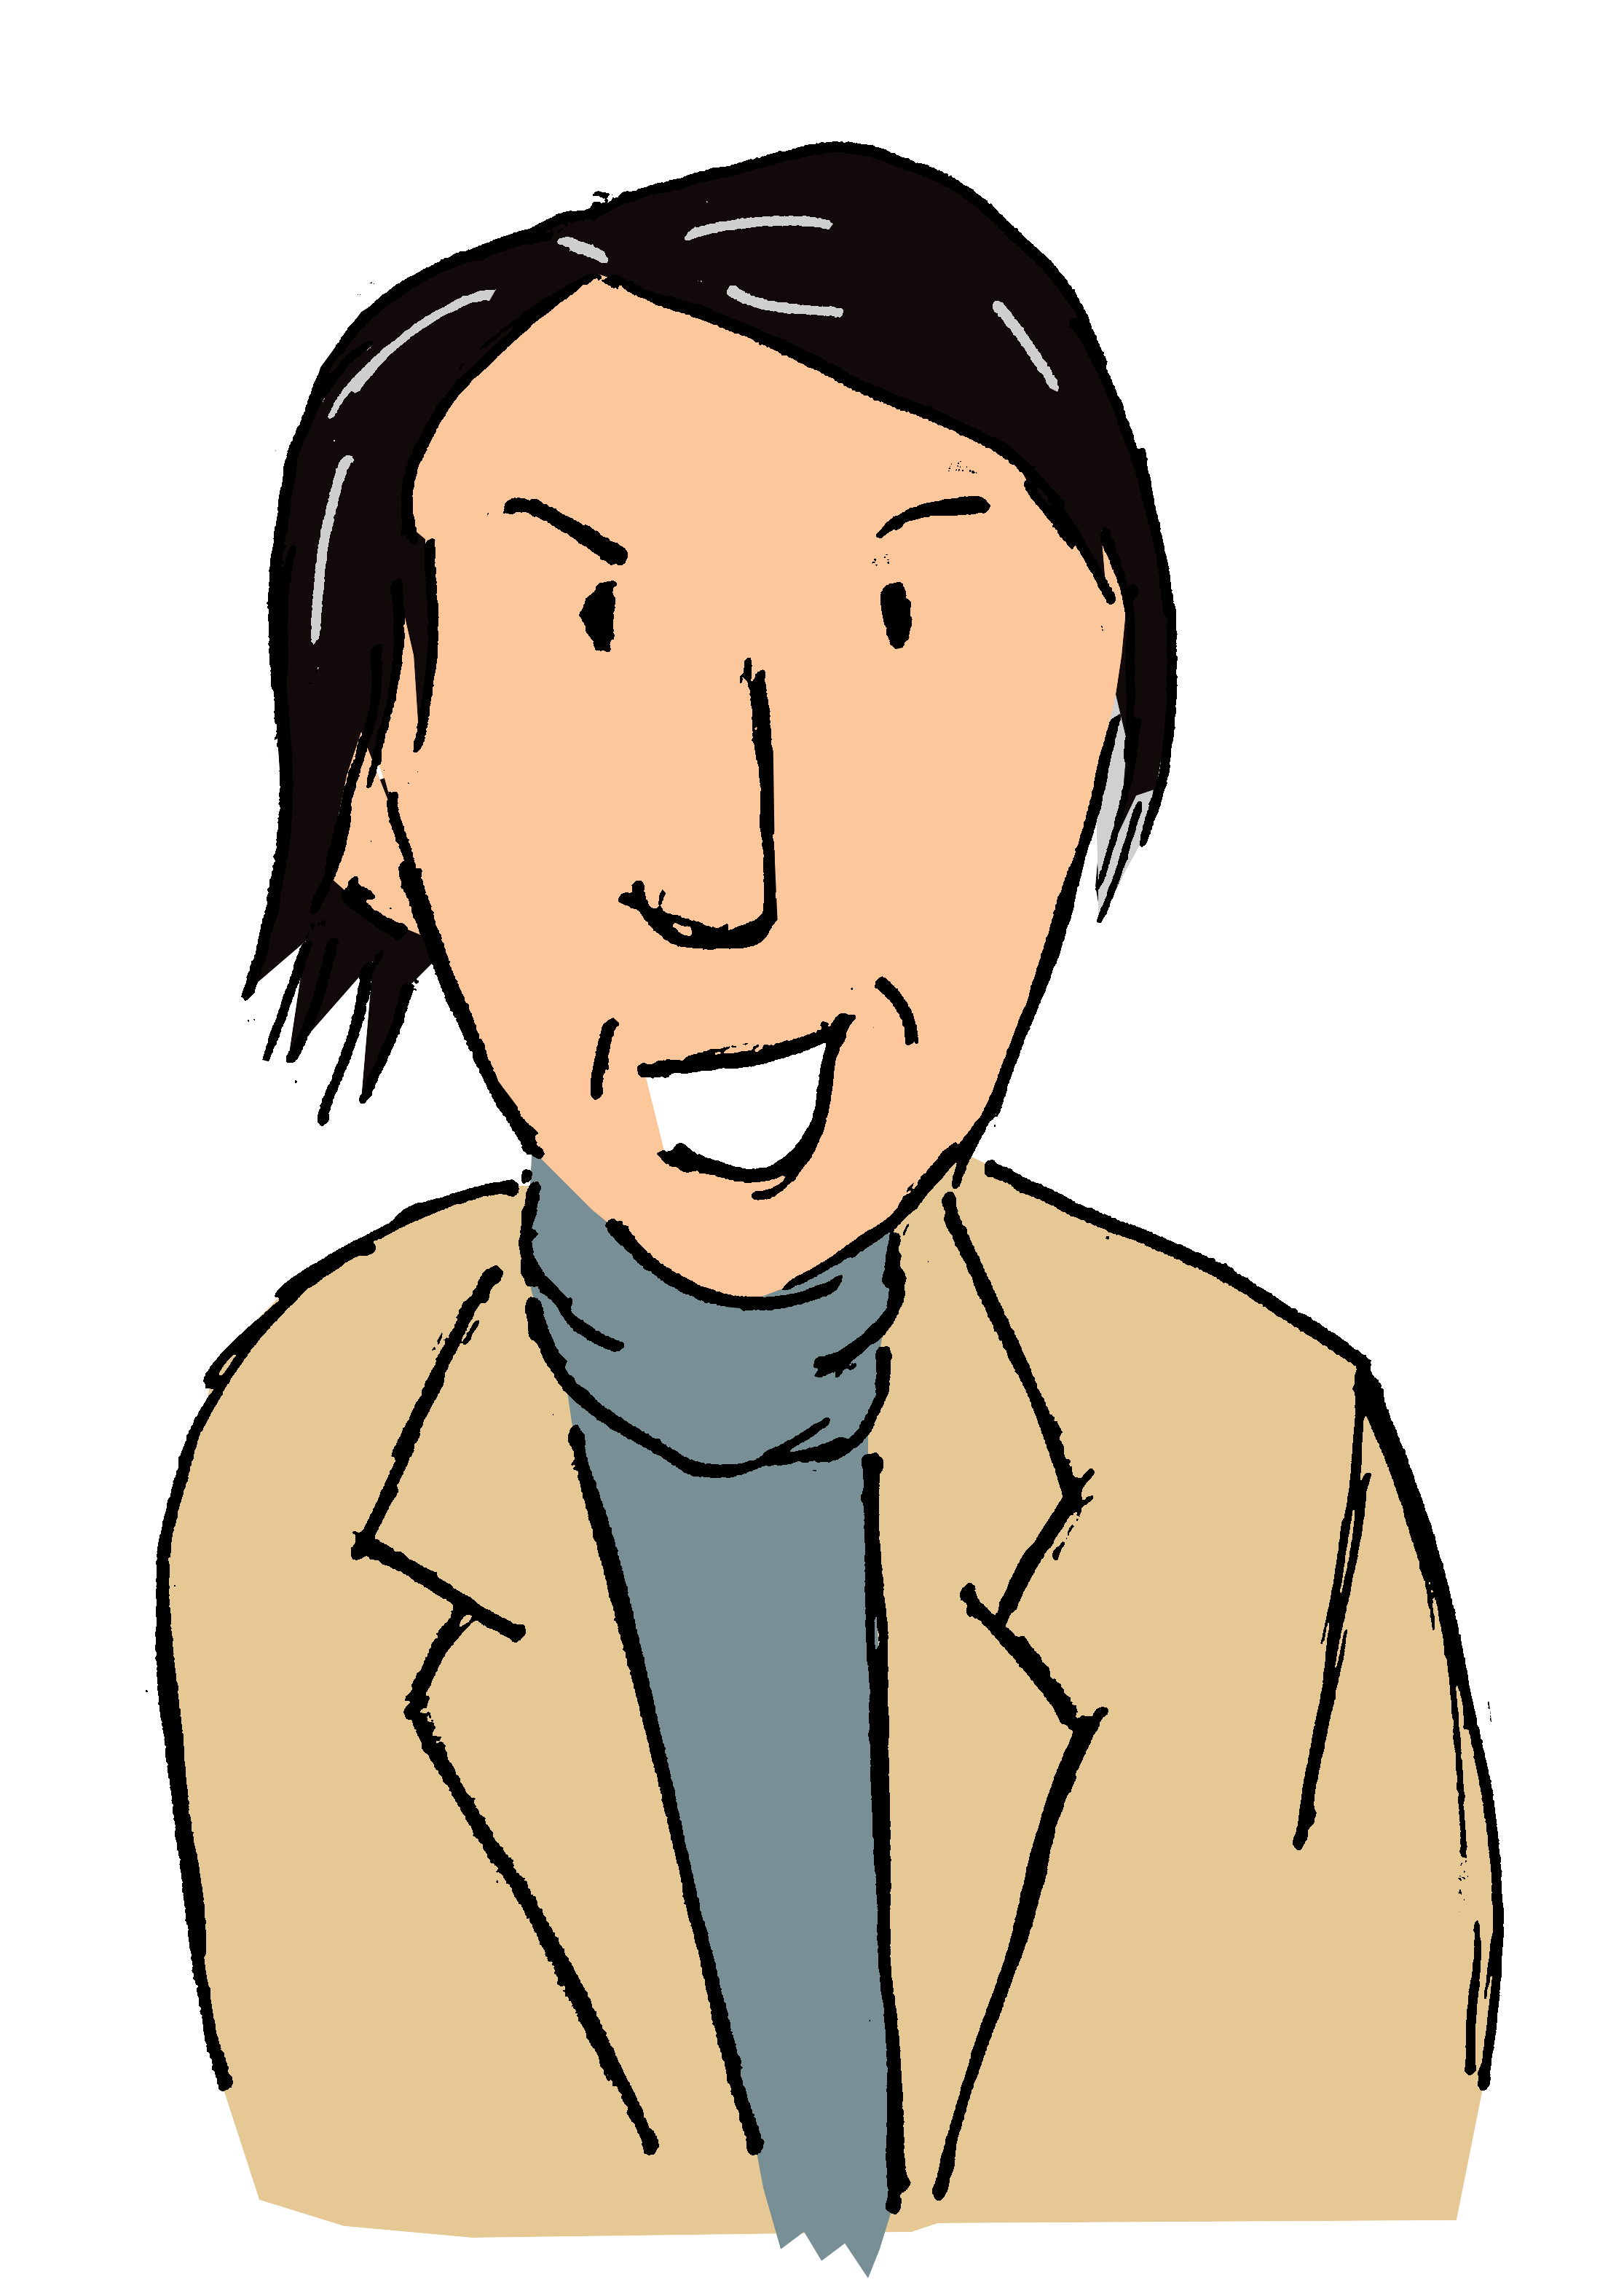
\includegraphics[width=5cm]{carl_sagan}};
			\node (example-textwidth-2) [notice={(3,0.5)}, ultra thick, right, align=center, text width=12cm, color=black, fill=white, font=\fontsize{23pt}{24pt}\selectfont] at (1,-1) {Vediamo ora tre differenti tipi di curve relativi a tre differenti tipi di moti nello spaziotempo:};
		\end{scope}
		%
		\begin{scope}[shift={(0,-90)}]
			\draw[fill=space,ultra thick] (0.5,7.5) rectangle (29,-5.5);
			\draw [->,color=white,ultra thick] (3,1) -- (15,1);
			\draw [->,color=white,ultra thick] (4,-4) -- (4,6);
			%
			\draw [color=white,ultra thick] (7,-3) -- (7,5);
			\draw [color=white,ultra thick] (9,-3) -- (11,5);
			\draw [color=white,ultra thick] (12,-3) to[out=90,in=214] (14,5);
			%
			\node at (16,1) {\textcolor{white}{\fontsize{23}{24}\selectfont x}};
			\node at (3,6) {\textcolor{white}{\fontsize{23}{24}\selectfont t}};
			%
			\node at (7,-4) {\textcolor{white}{\fontsize{23}{24}\selectfont a}};
			\node at (9,-4) {\textcolor{white}{\fontsize{23}{24}\selectfont b}};
			\node at (12,-4) {\textcolor{white}{\fontsize{23}{24}\selectfont c}};
			%
			\node (example-textwidth-2) [right, align=left, text width=11cm, color=white, font=\fontsize{23pt}{24pt}\selectfont] at (18,2) {La linea a rappresenta una particella a riposo, la linea b una particella che si muove a velocità costante e la curva c rappresenta una particella che si muove di moto accelerato.};
		\end{scope}
		%
		\begin{scope}[shift={(0,-100)}]
			\draw [ultra thick, fill=earth] (4.5,4) rectangle (9.5,-4);
			\node at (7,0) {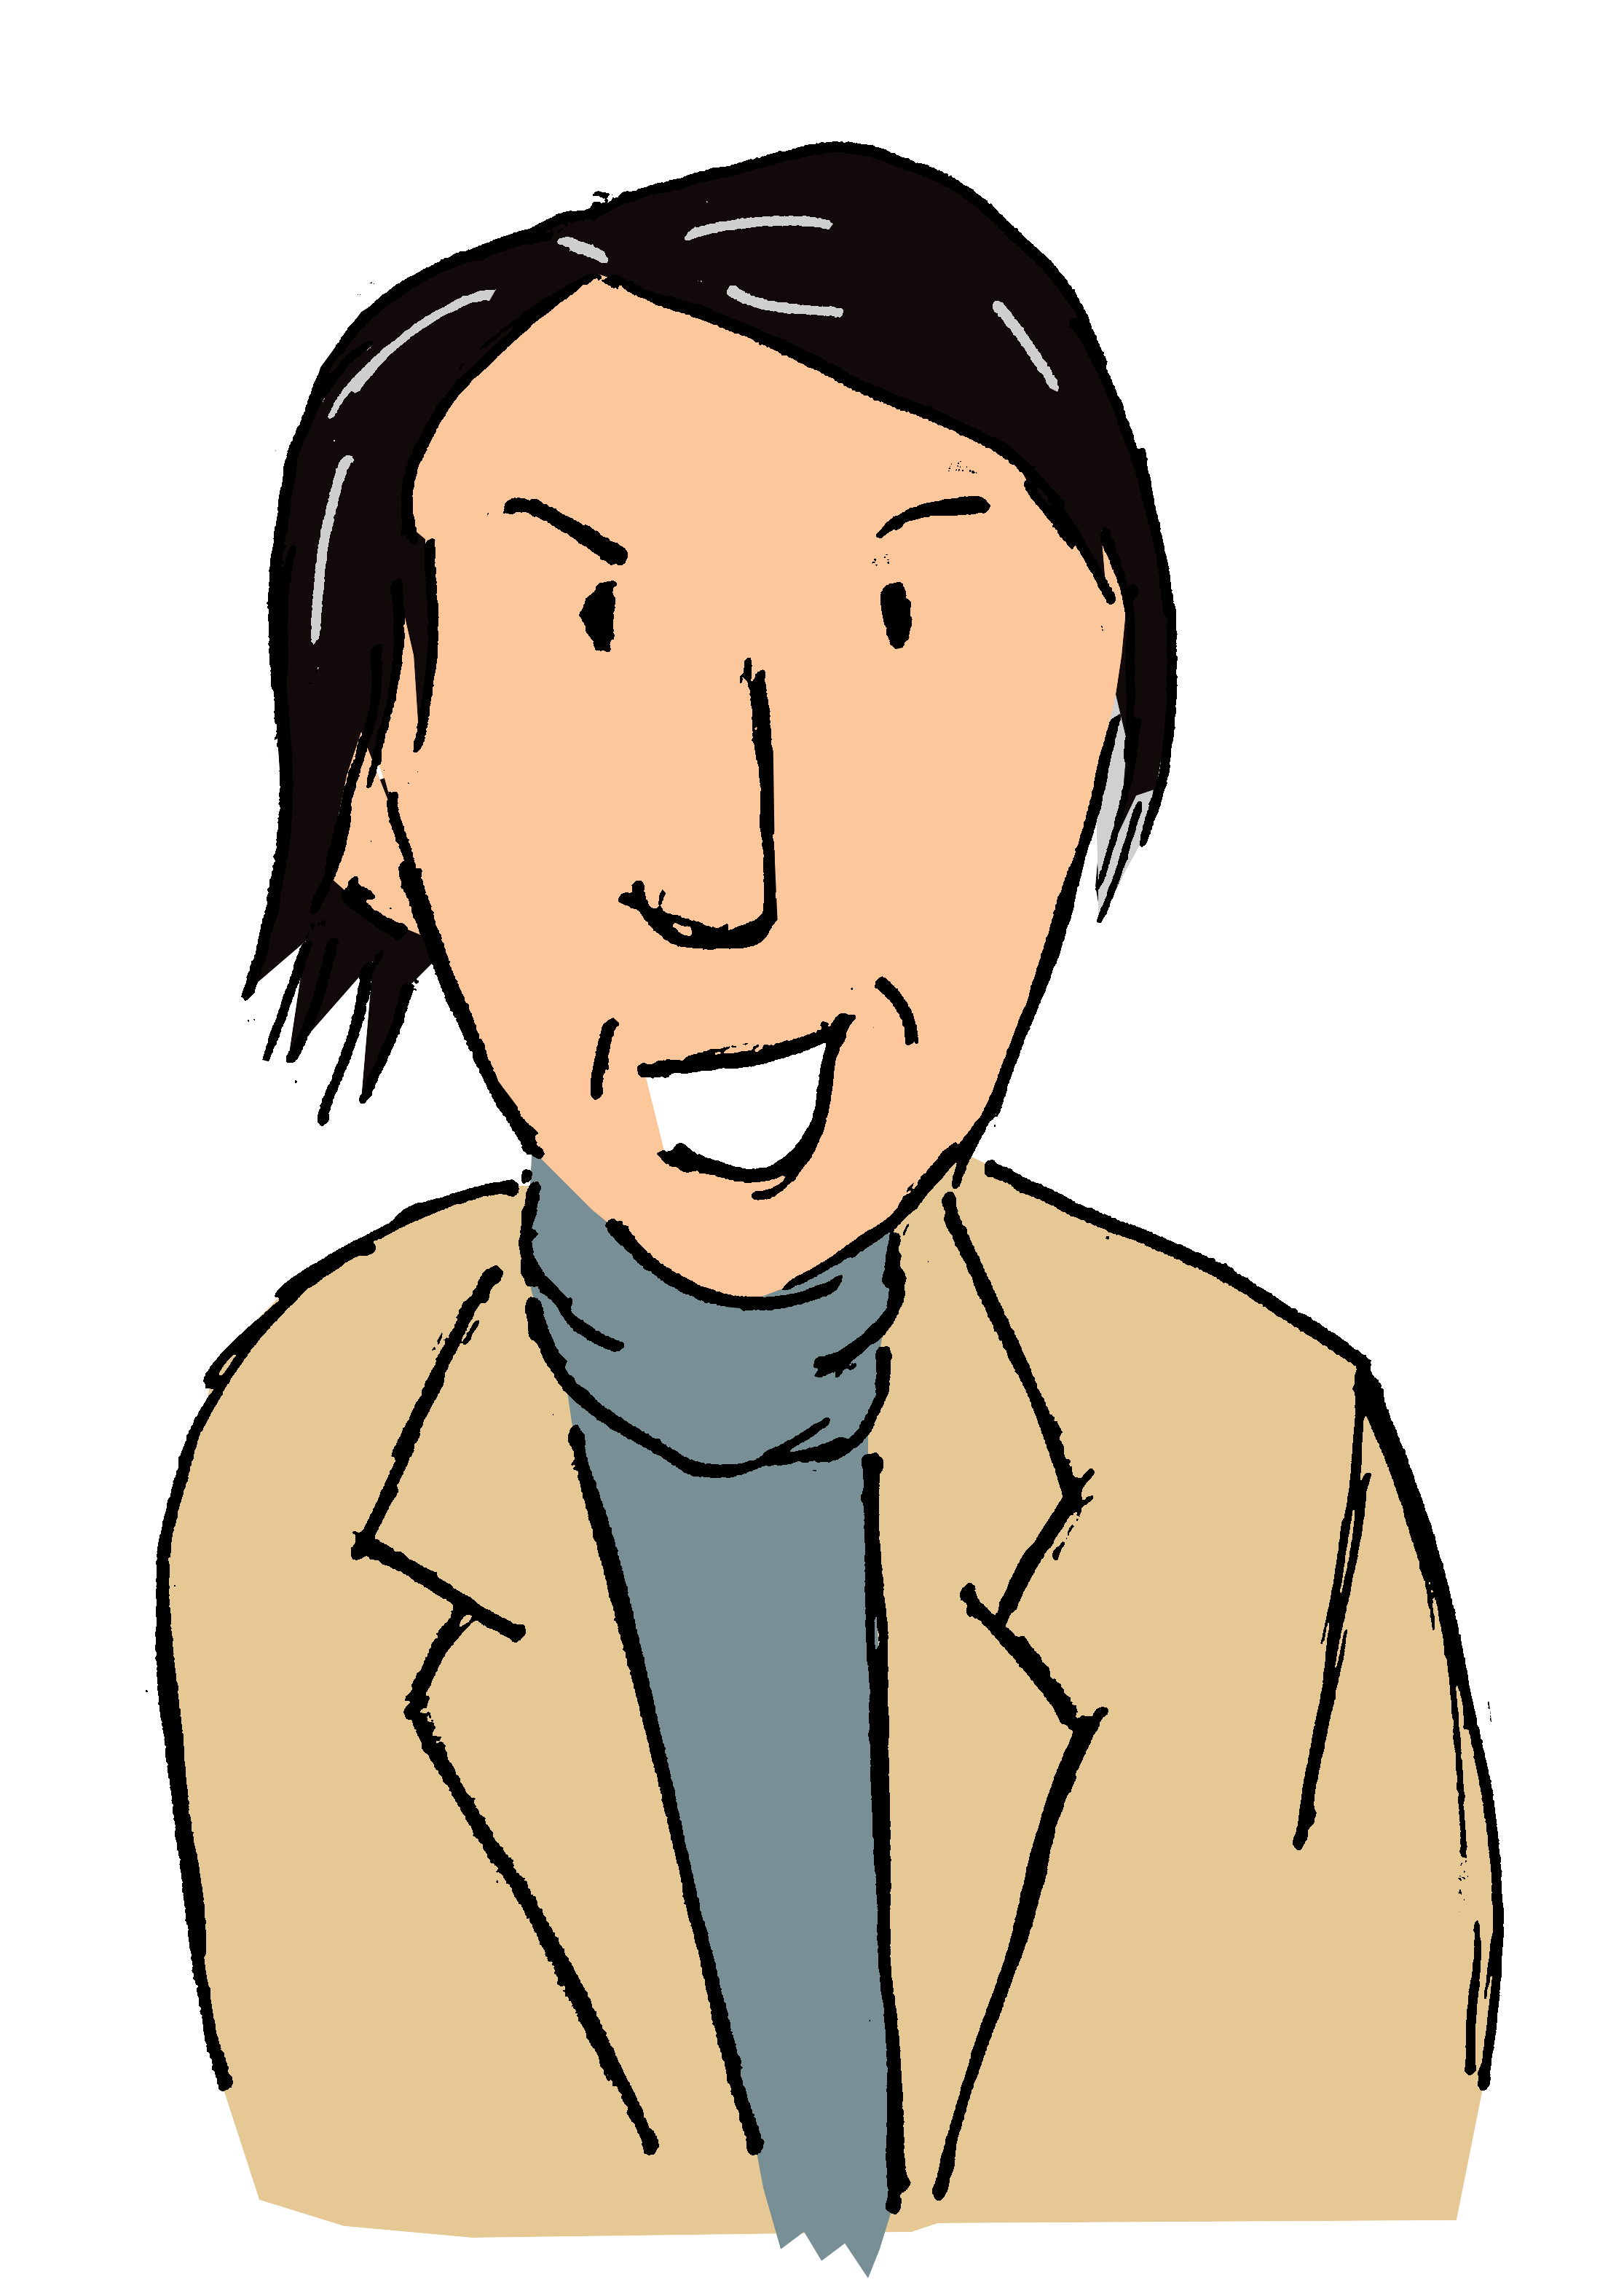
\includegraphics[width=5cm]{carl_sagan}};
			\node (example-textwidth-2) [notice={(-3,0.5)}, ultra thick, right, align=center, text width=12cm, color=black, fill=white, font=\fontsize{23pt}{24pt}\selectfont] at (12,-1) {Dunque l'arco di circonferenza tra Ottawa e Venezia, che in un certo senso rappresenta il moto dell'aereo nel campo gravitazionale della Terra, può essere una analogia alternativa per descrivere la deformazione dello spaziotempo generata dalla massa dei pianeti.};
		\end{scope}
		%
		\begin{scope}[shift={(0,-110)}]
			\node at (27,0) () {
\includegraphics[width=3.7cm]{licenza}};
			\node at (18,-0.1) {\textcolor{black}{\fontsize{14}{15}\selectfont Testo e illustrazioni: @ulaulaman - Gianluigi Filippelli}};
		\end{scope}
	\end{tikzpicture}
%
\end{document}
